\section{Architektur}
In dieser Arbeit kann kein komplettes Data-Lake-System entworfen werden.
Es muss aber eine Entscheidung getroffen werden, nach welcher Architektur das System aufgebaut werden soll.
Damit zuverlässig die Änderungen in einer Datenquelle erkannt werden können, dürfen die Daten, die von der Ingestion geschrieben wurden, nicht direkt verändert werden.
Hierfür wären sowohl die Zonen- als auch die Ponds-Architektur geeignet.
Beide können auch als eine datenorientierte Architektur bezeichnet werden.
Für die Implementierung des Data Lake soll eine Microservice-Architektur zum Einsatz kommen.
Daraus folgt, dass hier ebenfalls eine Aufteilung nach Funktionen der Komponenten notwendig ist.
Daher reicht eine pure datenorientierte Architektur des Data Lake nicht aus.
Am besten eignet sich in diesem Fall die von \textcite{sawadogo2021data} beschriebene hybride Architektur.

\subsection{Zonen-Architektur}
Von \textcite{ingestion_02} wurde eine Architektur basierend auf drei Zonen entwickelt.
\begin{enumerate}
    \item In der Drop Zone werden alle Daten ohne weitere Verarbeitung gespeichert.
          Nur die Datenproduzenten haben Zugriff auf diese Zone und können Daten schreiben.
    \item Die Landing Zone ist ein unveränderlicher Speicher, der Daten-Assets enthält, die jeweils zu einer Daten-Sammlung gehören. Projekte können mit den Assets aus der Landing Zone interagieren.
          Benutzer müssen lesenden Zugriff auf bestimmte Assets über einen Governance-Prozess beantragen.
    \item Projekte können in der Integration-Zone angereicherte Daten speichern.
          Diese Anreicherung kann zum Beispiel aus einer Aufarbeitung oder Umstrukturierung bestehen, die speziell für ein Projekt benötigt wird.
          Es ist außerdem möglich Daten aus der Drop Zone wieder in die Landing Zone zu laden.
\end{enumerate}
Zu diesem Zeitpunkt kann noch keine Aussage darüber getroffen werden, ob diese Architektur für die komplette Umsetzung des Data-Lakes geeignet ist.
Der Ansatz der Drop Zone jedoch, in der nur Datenproduzenten schreiben können, erfüllt genau die Bedingung, dass die Daten der Ingestion nicht durch andere verändert werden dürfen.
Es ist hier wichtig, dass die Daten mit denen neue Daten verglichen werden, seit der letzten Ingestion nicht verändert wurden, um genaue Aussagen über die geschehenen Änderungen in der Datenquelle treffen zu können.
Daher wird zumindest eine Zonen-Architektur mit der Drop-Zone für den Entwurf übernommen.
Die Datenproduzenten, in diesem Szenario, sind alle Microservices, die für die Speicherung von Daten zuständig sind.
Die Aufteilung in Funktionen kann ebenfalls noch nicht abgeschlossen werden, da in dieser Arbeit die Ingestion-Schnittstelle nur als die erste Funktion entwickelt wird.
Weitere Funktionen werden erst im Verlauf der Entwicklung hinzugefügt.
Dabei muss aber immer mit überlegt werden, ob neben den Funktionen auch weitere Zonen in der Data-Lake-Architektur hinzugefügt werden.

\subsection{Microservice-Architektur}
\label{sec:arch}

Neben der Architektur des Data Lake muss auch eine Architektur für die Microservices entworfen werden.
Diese legt fest, welche Komponenten benötigt werden, welche Aufgaben sie bearbeiten und wie sie miteinander interagieren.
Der erste Schritt dabei ist es, trennbare Aufgaben zu identifizieren und aufzuteilen.
Der Aufbau der Microservice-Architektur kann entweder funktions- oder prozessorientiert angegangen werden.

Bei einem funktionsorientierten Aufbau wird das System in einzelne Funktionen unterteilt.
Teile dieser Unterteilung können dann einzelnen Microservices zugewiesen werden.
Für die Ingestion-Schnittstelle sind das die Funktionen zum Laden der Daten, für die Deltaberechnung und zur Speicherung der Daten.
Da diese aber ein zusammenhängender Arbeitsablauf sind, der in einem Spark-Job ausgeführt werden kann, sollten diese auch nicht auf verschiedene Microservices aufgeteilt werden.

Hier ist der prozessorientierte Ansatz besser geeignet.
Dabei werden die technischen Abläufe betrachtet, um eine Unterteilung abzuleiten.
Bei der Ingestion-Schnittstelle lassen sich ergeben sich die API, das kontinuierliche Ausführen und die Ausführung der Ingestion mit Spark.
In \cref{fig:system-architektur} ist die Architektur für die Ingestion-Schnittstelle dargestellt.

Bei dem \textbf{API-Service} handelt es sich um den Service für die Interaktion mit dem Data-Lake-System.
Durch \nameref{ANF_14} ergibt sich, dass dieser ein Web-Server mit einer REST-API ist.
Es geht zwar in dieser Arbeit nur um die Ingestion, aber der API-Service sollte Schnittstellen zu allen Funktionen des Data-Lake-Systems enthalten.

Der \textbf{Ingestion-Service} ist dafür zuständig, die Datenquellen zu verarbeiten und den kompletten Prozess vom Laden bis zum Speichern der Daten in Apache Spark auszuführen.
Die Ingestion soll für eine Datenquelle nur einmal gleichzeitig, aber parallel für unterschiedliche Datenquellen ausgeführt werden können.

Bei einer zeitgesteuerten oder Datenstrom-Ingestion muss die kontinuierliche Ausführung sichergestellt werden.
Das wird durch den \textbf{Continuation-Service} übernommen.
Für alle Datenquellen muss regelmäßig geprüft werden, ob für diese gerade eine Ingestion ausgeführt wird und ausgeführt werden sollten.
Falls keine Ingestion ausgeführt wird, aber ausgeführt werden sollte, wird die Ingestion für diese Datenquelle gestartet.

Neben diesen Mircoservices wird noch ein Nachrichtensystem benötigt.
Das Nachrichtensystem stellt die Kommunikation zwischen den Microservices dar.
Hier ist es wichtig, dass es einem Sender möglich ist, Nachrichten an einen oder auch an mehrere Empfänger zu senden.
So soll sichergestellt werden, dass bestehende Microservices einfach repliziert und neue eingefügt werden können.
Für das Speichern von Daten und Metadaten wird jeweils ein Speichersystem benötigt.

\begin{figure}
    \centering
    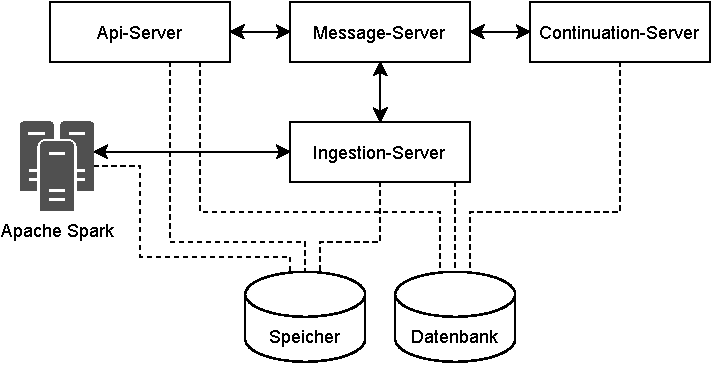
\includegraphics{Grafiken/Entwicklung-System-Architektur.pdf}
    \caption{Microservice-Architektur der Ingestion}
    \label{fig:system-architektur}
\end{figure}
